%\documentclass[aps,prb,superscriptaddress,showpacs,reprint]{revtex4-1}
\documentclass[3p,twocolumn]{elsarticle}
\usepackage{fullpage}
\usepackage{amsfonts}
\usepackage{amssymb}
\usepackage{amsmath}
\usepackage{hyperref}
\usepackage{graphicx}% Include figure files
\usepackage{epstopdf}
\usepackage{subfig}
\usepackage[normalem]{ulem}
\begin{document}
%\usepackage{setspace}\doublespace
\title{Competition between BCS-pairing and moth-eaten effect in BEC-BCS crossover}
\author[uiuc]{Guojun Zhu\corref{cor1}}
%\affiliation{Department of Physics, University of Illinois at Urbana-Champaign, 1110 W Green St, Urbana, IL, 61801}
\ead{gzhu1@illinois.edu}
\author[uiuc,upmc]{Monique Combescot}
\ead{Monique.Combescot@insp.jussieu.fr}
%\affiliation{Institut des NanoSciences de Paris, Universite Pierre et Marie Curie, CNRS, Tour 22, 4 place Jussieu, 75005 Paris }
%\affiliation{Department of Physics, University of Illinois at Urbana-Champaign, 1110 W Green St, Urbana, IL, 61801}

%\affiliation{Department of Physics, University of Illinois at Urbana-Champaign, 1110 W Green St, Urbana, IL, 61801}
\address[uiuc]{Department of Physics, University of Illinois at Urbana-Champaign, 1110 W Green St, Urbana, IL, 61801}

\address[upmc]{Institut des NanoSciences de Paris, Universite Pierre et Marie Curie, CNRS, Tour 22, 4 place Jussieu, 75005 Paris }
%\cortext[cor1]{+1-217-3335224}
\newcommand{\vk}{\ensuremath{\mathbf{k}}}
\newcommand{\vK}{\ensuremath{\mathbf{K}}}
\providecommand{\vr}{\ensuremath{\mathbf{r}}}
%\newcommand{\vec}[1]{\ensuremath{\mathbf{#1}}}

\newcommand{\gk}{\ensuremath{{g}(\mathbf{k})}}

\newcommand{\vp}{\ensuremath{\mathbf{p}}}
\newcommand{\gp}{\ensuremath{{g}(\mathbf{p})}}

\newcommand{\vq}{\ensuremath{\mathbf{q}}}

\newcommand{\Fo}{\ensuremath{\mathbf{F_0}}}


\newcommand{\E}{\ensuremath{\mathbf{E}}}
\newcommand{\A}{\ensuremath{\mathbf{A}}}
\newcommand{\J}{\ensuremath{\mathcal{J}}}

\newcommand{\ket}[1]{\ensuremath{\left|#1\right>}}
\newcommand{\bra}[1]{\ensuremath{\left<#1\right|}}

\newcommand{\twoe}{\ensuremath{2\epsilon_\vk-\E_1}}

\newcommand{\nth}[1]{\ensuremath{\frac{1}{#1}}}

\newcommand{\br}[1]{\ensuremath{\left(#1\right)}}
\newcommand{\mbr}[1]{\ensuremath{\left[#1\right]}}
\newcommand{\bbr}[1]{\ensuremath{\left\{#1\right\}}}


\newcommand{\tk}{\ensuremath{\tilde{k}}}

\newcommand{\kp}{\ensuremath{\ket{\Psi}}}

\newcommand{\av}[1]{\ensuremath{\bigl<{#1}\bigr>}}
\newcommand{\avs}[3] {\av{#1{\lvert{#2}\rvert}#3}}
\newcommand{\avv}[2][\nu] {\avs{#1}{#2}{#1}}
\newcommand{\avt}[2]{\av{{#1}|{#2}}}
\newcommand{\avtu}[1]{\av{T_\tau#1}}

\newcommand{\Bop}{\ensuremath{\mathbf{B_0^+}}}
\newcommand{\Bmp}{\ensuremath{\mathbf{B_m^+}}}
\newcommand{\Bnp}{\ensuremath{\mathbf{B_n^+}}}
\newcommand{\Bo}{\ensuremath{\mathbf{B_0}}}
\newcommand{\Bopn}{\ensuremath{\mathbf{{B_0^+}^n}}}
\newcommand{\Bon}{\ensuremath{\mathbf{{B_0}^n}}}


\newcommand{\zmatrix}{\ensuremath{\br{\begin{smallmatrix}0&0\\0&0\end{smallmatrix}}}}
\newcommand{\fmtrx}[4]{\ensuremath{\br{\begin{smallmatrix}#1&#2\\#3&#4\end{smallmatrix}}}}
\newcommand{\smtrx}[6]{\ensuremath{\br{\begin{smallmatrix}#1&#2\\#3&#4\\#5&#6\end{smallmatrix}}}}

\newcommand{\vz}{\ensuremath{v^{\beta\alpha}_{\vk,\vk}}}
%\newcommand{\fz}{

\providecommand{\abs}[1]{\ensuremath{\lvert{#1}\rvert}}

\newcommand{\sg}[1][1]{\ensuremath{\sigma_\frac{#1}{2}}}

\newcommand{\rhof}{\ensuremath{\rho(\ef)}}
\newcommand{\omt}{\ensuremath{\tilde{\Omega}}}
\newcommand{\cht}{\ensuremath{\tilde{\chi_0}}}
\newcommand{\Atl}{\ensuremath{\abs{A}^{2l}}}
\newcommand{\ef}{\ensuremath{\epsilon_F}}

\newcommand{\lca}{\ensuremath{\ln\br{1+\frac{\cht}{\alpha}}}}

\newcommand{\com}[2]{\ensuremath{\mbr{#1,#2}}}
\newcommand{\D}{\ensuremath{\mathit{D}}}
\newcommand{\dg}{\ensuremath{\dagger}}

\providecommand{\lvk}{\ensuremath{1/\vk_F}}
\providecommand{\hm}{\ensuremath{\frac{\hbar^2}}{2m}}
\providecommand{\pdiff}[2]{\ensuremath{\frac{\partial{#1}}{\partial{#2}}}}
\providecommand{\dpdiff}[2]{\ensuremath{\frac{\partial^2{#1}}{\partial{{#2}^2}}}}

\providecommand{\H}{\ensuremath{\mathcal{H}}}
\providecommand{\wt}[1]{\widetilde{#1}}

\providecommand{\eef}[1]{Eq. (\ref{#1})}

\providecommand{\sch}{{Schr\"{o}dinger }}

\providecommand{\sgn}{\ensuremath{\text{sgn}}}


\providecommand{\comm}[1]{\textit{\scriptsize \uwave{(#1)}}}
\newcommand{\td}{{\ensuremath{{\text{(2D)}}}}}
\newcommand{\sd}{{\ensuremath{{\text{(3D)}}}}}
\newcommand{\Arctg}{\ensuremath{\text{Arctg}}}



\numberwithin{equation}{section}
\begin{abstract}
We study the evolution of the condensation energy induced in cold gases by the  reduced BCS hamiltonian from single pair of fermions to large amount of pairs in thermodynamic limit.  We observe that absolutely amount of energy-saving due to pairing decreases while pair number increases because the phase space for each additional pair gets smaller (moth-eaten effect).  However, comparing to the increase of kinetic energy as free Fermi gas, this decrease is smaller at first and only dominates  when total number of particles is close to the total available states.  
\end{abstract}
\begin{keyword}
A.Superconductor; D.Cooper Paring; D.Crossover
\end{keyword}

\maketitle
\section{Introduction}
It was known for a long time that a 3D system having a weak attractive potential cannot sustain a bound-state.  In 1956, Cooper showed that in the presence of a frozen Fermi sea, a pair of electrons with opposite spin can form a bound-state of zero total momentum  no matter how weak the attraction is\cite{Cooper}.  This state actually is indeed a many-body state because the  Fermi sea, even if it does not interact through the reduced BCS potential,  is essential for the formation of ``two-body'' bound state.   The next year, Bardeen, Cooper and Schrieffer introduced a many-body ansatz which is an extension of this single pair ``bound state'' and showed that this ansatz gives an intricate many-body state with lower energy than free Fermi gas with arbitrarily weak attraction\cite{BCS} for the same reduced BCS hamiltonian.  They used a particle-number non-conserved ansatz in a grand-canonical ensemble.  Nevertheless, the reduced BCS model also has a frozen Fermi sea in the core. Later,   Gor'kov and Melik-Barkhudarov showed that the frozen Fermi sea is not necessary and the same idea works with a renormalized attraction measured by low energy scattering amplitude\cite{Gorkov}.   Furthermore, Eagles\cite{Eagle}, Leggett\cite{LeggettCrossover}, Nozi\`{e}res and Schmitt-Rink\cite{Nozieres} extended the BCS pairing idea and bridged Cooper pairing and molecular BEC. There they used the model without a frozen Fermi sea as core and employed the full k-space.  All these lead to an interesting question that how the solution for the same hamiltonian evolves from one-pair, where there might be no bound state, to infinite number of pairs, where a many-body bound solution always exists.  Nevertheless, the particle non-conserved nature of the BCS ansatz makes it inherently many-body, which is quite difficult to connect to one-pair solution.  

Five years after BCS, Richardson showed that a number-conserved eigenstate exists for the reduced BCS Hamiltonian and it gives the same energy as BCS ansatz in thermodynamic limit\cite{Richardson1,Richardson2,Richardson3,Richardson1968,gaudin}.  In the model, a frozen Fermi sea also exists in order to provide a constant density of states.  Since 2000, we developed a new theoretical framework for composite bosons (cobosons for short) formed by fermion pairs for electron excitons\cite{CobosonPhysicsReports}.   Recently, we applied it into superconductivity and it was proved to be useful.  We rederived Richardson-Gaudin equations with coboson framework\cite{CobosonBcsRich}. We also studied Richardson equations in details \cite{CombescotCooper,combescotBCS}.  Richardson-Gaudin solution, as a number-conserved one, is  particular suitable to investigate the question we raised.  

It is illuminating to image the additional pair was added to the system of few tightly-bound pairs.   Pauli exclusion would show in two different places roughly speaking.  (i) Pairing (binding) happens in more restricted phase space, and therefore the energy saving by potential becomes less than the previous pair, which enjoy larger phase space.  This is the moth-eaten effect we discussed in exciton context extensively\cite{CobosonPhysicsReports}.  (ii) On the other hand, in free fermion gas where there is no attraction, the extra fermions has to piled in the next k-level and also cost more energy due to Pauli exclusion.  Of course, these two effects must be solved in a self-consistent fashion.  We will do that in sec. \ref{sec:twoPair}.  Nevertheless, it is useful to separate them in order to build some intuition on the problem.  In a 3D system with strong attraction, we can estimate the first effects from our previous work in exciton, the energy decrease is in order of $N\frac{a^3}{V}$, where $N$ is the total number of pairs, $a$ is the average size of pair in two-body Schr\"{o}ndinger equation, and $V$ is the volume of the system. The second effect is in order $1/\rho(\epsilon_F)$, where $\rho(\epsilon)\sim\sqrt{\epsilon}$ is the density of the state, $\epsilon_F\sim\left(\frac{N}{V}\right)^{2/3}$. So the new pair would cost energy in ordr of $\left(\frac{V}{N}\right)^{2/3}$. When $N$ is small, (ii) dominates (i). Therefore, the condensation energy, the difference between the system energy with potential and without potential (as free gas), increases.  And when $N$ gets larger and larger, (ii) increases not as fast as (i) and finally (i) dominates and condensation energy decreases.    This argument is somewhat hand-waving, yet the intuition here proves to be quite close to truth.  We will set them in solid ground in the following parts of the paper. 

We illustrate our model in sec. \ref{sec:model}.  In sec. \ref{sec:onePair}, we study the one-pair problems in detail for both 2D and 3D.  We discussed the N-pairs problems, and make some conjecture about their connection with one-pair solution  in sec. \ref{sec:NPair}.  And we will attempt 2-pair Richardson-Gaudin equations and put the conjecture into the solid ground in sec \ref{sec:twoPair}.  And we will offer some final thought in sec. \ref{sec:conclusion}.
\section{The model\label{sec:model}}
We consider $N$ fermion pairs with creation operators $a_\vk^\dagger$ and $b_\vk^\dagger$.  These fermions are  governed by the hamiltonian
\begin{equation}
H=H_{0}+V
\end{equation}
where  the kinetic part $H_0$ reads as 
\begin{equation}
H_0=\sum_{\vk}\epsilon_\vk(a^\dagger_\vk{}a^{}_\vk+b^\dagger_\vk{}b^{}_\vk)
\label{eq:}
\end{equation}
the interaction $V$ being taken as 
\begin{equation}
V=-v\sum_{\vk\vk'}w_{\vk'}w_\vk\beta^\dagger_{\vk'}{}\beta^{}_\vk
\label{eq:VBcs}
\end{equation}
 $\beta^\dagger_{\vk}=a^\dagger_{\vk}b^\dagger_{-\vk}$ creates a zero momentum pair while $w_\vk=1$ for $0<\epsilon_\vk<\Omega$ and zero otherwise.  The potential we take in this model, is the reduced BCS  potential without an inside frozen Fermi sea, so that attraction starts from zero to a sharp cutoff $\Omega$.  As a result,  $\Omega$ bears no connection with the Debye energy as in the original BCS model. This potential extension $\Omega$ can however relate to another physical quantity, namely, the scattering length %(see sec. \ref{sec:scatter}). \comm{It has a quite implicit relation to scattering length. Are we going to include this relation in the paper?}
\section{One pair\label{sec:onePair}}
Let us start with a single pair. Its energy $E_1$ follows from Cooper's equation
\begin{equation}
1=v\sum_{\vk}\frac{\omega_\vk}{2\epsilon_\vk-E_1}\equiv{}v\,S(E_1)
\label{eq:onePair}
\end{equation}
\subsection{One pair in 2D systems}
In 2D system with negligible width, the density of state is constant, so that for negative solution to $E$ 
\begin{equation}
S^{(\text{2D})}(E<0)=\rho\int_0^{\Omega}\frac{d\epsilon}{2\epsilon-E}=\frac{\rho}{2}\ln\left(\frac{2\Omega-E}{-E}\right)
\label{eq:s1pair}
\end{equation}
\begin{figure}[htbp]
	\centering
		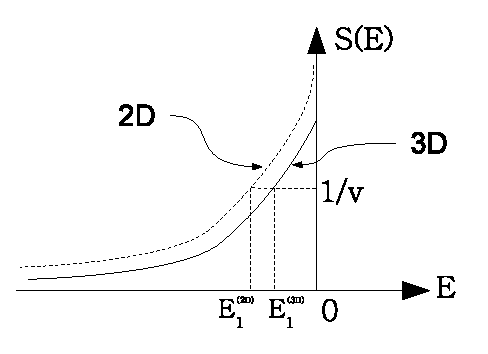
\includegraphics[width=0.30\textwidth]{OnePair.eps}
	\caption{$S^\td(E)$ and $S^{\sd}(E)$ function}
	\label{fig:OnePair}
\end{figure}
$S^{(\text{2D})}(E)$ goes to infinity when $E\rightarrow{}0_{-}$ while it goes to zero as $\rho\Omega/(-E)$ when $E$ goes to $-\infty$. Consequently, a bound state with $E_1<0$ solution of Eq. (\ref{eq:onePair}),  exists no matter how weak the potential amplitude $v$ is. It reads
\begin{equation}
E_1^{(\text{2D})}=-\frac{2\sigma}{1-\sigma}\Omega
\label{eq:}
\end{equation}
where we have set $\sigma=e^{-2/\rho{v}}$



\subsection{One pair in 3D systems}
In 3D, the density of states increases as $\sqrt{\epsilon}$. Let us write it as 
\begin{equation}
\rho(\epsilon)=\rho\sqrt{\epsilon/\Omega}
\label{eq:}
\end{equation}
where $\rho$ is the density of state at the potential upper boundary. As for 2D systems, $\rho$ is proportional to the sample volume.   Using this density of state, we find
\begin{equation}
\begin{split}
S^\sd(E<0)&=\rho\int_0^{\Omega}{}d\epsilon\frac{\sqrt{\epsilon/\Omega}}{2\epsilon-E}\\
	&=\rho(1-\sqrt{\frac{-E}{2\Omega}}\Arctg\sqrt{\frac{2\Omega}{-E}})
\label{eq:}
\end{split}
\end{equation}
$S^\sd(E)$ goes to $\rho$ when $E\rightarrow0_-$ while it goes to zero as $\frac{2}{3}\rho\Omega/(-E)$ when $E$ goes to $-\infty$. 
A bound state with $E_1<0$ thus exists for $v$ larger than a threshold value which for a single pair, $N=1$, is given by  $v_{\text{th}}(N=1)=1/\rho$.  For a potential just above threshold, the single pair energy in 3D tends to zero as 
\begin{equation}
E_1^\sd\approx-\frac{8}{\pi^2}\left(1-\frac{1}{\rho{}v}\right)^2\Omega
\label{eq:E3Dsmall}
\end{equation}
while for a potential far above threshold $E_1^\sd$ behaves as 
\begin{equation}
E_1^\sd\approx-\frac{2}{3}\rho{v}\Omega
\label{eq:E3Dlarge}
\end{equation}
Note that while $\rho$ increases linearly with the sample volume.  the product $\rho{v}$ stays constant. 

\section{N pairs\label{sec:NPair}}
Richardson \cite{Richardson1} and Gaudin \cite{gaudin} have shown that the energy of $N$ fermion pairs interacting through the BCS reduced potential  is  given by $E_N=R_1+\cdots+R_N$ where the $R_i$'s follow from $N$ coupled nonlinear equations 
\begin{equation}
 1=v\sum_\vk\frac{w_\vk}{2\epsilon_\vk-R_i}+\sum_{j\neq{}i}\frac{2v}{R_i-R_j}
\end{equation}
{for} $i=(1,\cdots,N)$.
\subsection{$N$ pairs in 2D systems}
Very recently, we have shown that when the density of states is constant, as in standard BCS superconductivity with a frozen Fermi sea but also in 2D systems, a compact form of $E_N$ exists. It  reads as  
\begin{equation}\label{eq:E2dN}
 E^\td_N=N\,E^\td_1+\frac{N(N-1)}{\rho}\frac{1+\sigma}{1-\sigma}
\end{equation}
within under-extensive terms in $(N/\rho)^n$ with $n\leq2$. This explain why these terms do not appear in thermodynamical limit, as obtained in the grand-canonical approach to the BCS condensation energy. 

If we now consider the condensation energy, i.e., the difference between the $N$-pair energy without and with potential, over the number of pairs, as 
\begin{equation}
 \mathcal{E}^{(2D)}_N=E_N^{\td}(v=0)-E_N^\td\equiv{}N\epsilon_N^\td
 \end{equation}
 Eq. (\ref{eq:E2dN}) shows that the condensation energy $\epsilon_{N}^{\td}$ per pair reduces in 2D to
 \begin{equation}
\epsilon^{(2D)}_N=(1-\frac{N-1}{N_\Omega})\frac{2\sigma}{1-\sigma}\Omega\label{eq:E2D}
\end{equation}
where for 2D system, the total number of states in the potential layer reads $N_\Omega=\sum{}w_{\vk}=\rho\Omega$. 

We see that in 2D systems, the condensation energy per pair $\epsilon^\td_N$  decreases linearly with $N$ over the whole density range. This decrease is due to a moth-eaten effect induced by Pauli blocking on the number empty states feeling the potential and thus available to from the $N$-pair bound state.  When the number of pairs fills the whole potential layer, $N=N_\Omega$, the condensation energy per pair reduces to 
\begin{equation}
 \epsilon^\td_{N_\Omega}=\frac{1}{\rho}[\frac{2\sigma}{1-\sigma}]
\end{equation}
so that it tends to zero as $1/\rho$ in the large sample limit: for $N=N_\Omega$, the system has  essentially lost all its freedom to construct a lower energy ground state, as in the case of partial feeling for ???? the condensation energy per pair stays finite when the sample volume increases.  


\begin{figure}[htbp]
	\centering
		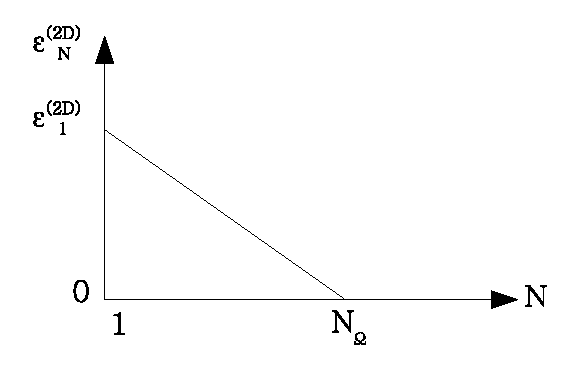
\includegraphics[width=0.30\textwidth]{2dCondEnergy.eps}
	\caption{Condensation energy per pair as a function of the pair number in 2D systems.}
	$N_{\Omega}=\rho\Omega$ is the total number of pair state in the potential layer
	\label{fig:2dCondEnergy}
\end{figure}



\subsection{$N$ pairs in 3D system}
Unfortunately, a  compact expression of the $N$-pair energy similar to Eq. (\ref{eq:E2dN}) has not been derived so far in the case of a $\sqrt{\epsilon}$ density of states. We are thus mostly left with a qualitative understanding of the $N$ pair energy  behavior when $N$ increases. 

First, it is clear that the same moth-eaten effect must bring the condensation energy per pair down to zero when $N$ approach the total number of pair in the potential layer which for 3D systems now reads $N_\Omega=\sum_{\vk}w_{\vk}=\frac{2}{3}\rho\Omega$. This moth-eaten effect is fundamentally linked to  Pauli blocking , so that it must stand unaffected by an increase of space dimensionality. 

\subsubsection{$v$ below threshold for single pair}
For a potential $v$ lower than the threshold value for single pair $v_{th}(1)=1/\rho$, the condensation energy per pair $\mathcal{E}_N^\sd$ is equal to zero for $N=1$ and also for $N=N_\Omega$.  It is however clear that $\mathcal{E}_N^\sd$ cannot stay equal to zero for all $N$ between $1$ and $N_\Omega$ because when $N$ becomes equal to a fraction of $N_\Omega$, the density of states is essentially constant.  So that we can always think of  freezing a small fraction of these electrons as in standard BCS superconductivity with a frozen Fermi sea: a finite condensation energy then  appears no matter how weak $v$ is. 

\begin{figure}[htb]
	\centering
		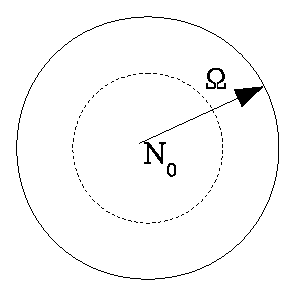
\includegraphics[width=0.20\textwidth]{potential.eps}
	\caption{Effective frozen core in the case of many pairs in 3D system}
	\label{fig:potential}
\end{figure}

To have an estimate of this condensation energy, let us freeze $N_0$ of these $N$ electrons, $\epsilon_{F_{0}}$ being the corresponding Fermi energy.  The remaining $N-N_0$ pairs enjoy the potential attraction in a region where the density of state stays finite, between $\rho\sqrt{\epsilon_{F_0}/\Omega}$ and $\rho$.  The condensation energy of these $(N-N_0)$ pairs would then read according to Eq. (\ref{eq:E2D})
\begin{equation}\label{eq:E3D}
{\mathcal{E}}_{N-N_0}=(N-N_0)(1-\frac{N-N_0-1}{N_\Omega})\frac{2\bar\sigma}{1-\bar\sigma}\Omega
\end{equation}
where $\bar{\sigma}=e^{-2/{\bar{\rho}v}}$ with $\bar\rho$ being the average density of states in the potential layer above the frozen core that we are going to approximate by $\rho$. This condensation energy is maximum for $N-N_0=N_\Omega/2$, which implies  $N$ substantially larger than $N_\Omega/2$.

This argument essentially shows that, even if $N$ is not as large as $N_\Omega/2$, but still a sizable faction of the total number of pair state $N_\Omega$ feeling the potential,  a BCS-like collective effect  must take place to produce a non-zero condensation energy, no matter how weak the potential is, i.e., even for $v\ll{}v_\text{th}(1)$. 

As a result, the threshold potential for the appearance of a $N$-pair condensation  must decrease with $N$, down to essentially zero when $N$ is a sizable fraction of the total number of pairs $N_\Omega$ in the potential layer.  As shown in Fig. \ref{fig:3dCondChange}, the condensation energy per pair must then increases until $N$ ultimately decreases to zero due to the moth-eaten effect which takes place when most pair states available to form the condensate are occupied. 


\begin{figure}[htb]
	\centering
		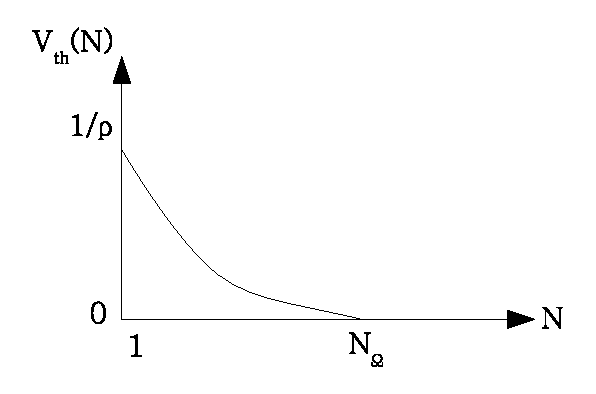
\includegraphics[width=0.30\textwidth]{3dThresholdChange.eps}
	\caption{Threshold change against number of pairs in 3D}
	\label{fig:3dThresholdChange}
\end{figure}

\subsubsection{$v$ above threshold in single pair}
For $v$ above the single pair threshold potential $v_{\text{th}}(1)=1/\rho$, it becomes  clear by continuity, that the condensation energy per pair $\epsilon^\sd_N$, must first increases with $N$ and then decreases due to the same moth-eaten effect which ends by controlling the condensation energy behavior when $N$ approaches full filling.  

Although fully reasonable, this continuity argument is a mathematical argument. Let us now grasp the physical origin of the condensation energy increase when $N$ increases above 1 for a potential larger than $v_{\text{th}}(1)$.  For that, we have to remember that the condensation energy is the difference of two energies which both increase with $N$ due to Pauli blocking.  The question then is to understand why, for small $N$, the free pair energy increases faster than the correlated pair energy.  (i) When one free pair is added at the energy level $\epsilon$, the kinetic energy increases by $1/\rho(\epsilon)$.  As a result, in 3D systems with a density of states in $\sqrt{\epsilon}$, the free pair energy change when going from $N$ to $N+1$ pairs, is  larger for low energy states.  (ii) By contrast, correlated pairs are made of all pairs in the potential layer. When increasing their number from $N$ to $N+1$, we blocks a very small fraction of each of the states between $0$ and $\Omega$, so that the energy change must be far less than when blocking a single low energy state.  Consequently, when $N$ is small,  the energy difference when adding one free pair or one correlated must increase with $N$. When $N$ gets large, the cost in energy $1/\rho(\epsilon)$ to add one free pair is essentially constant and equal to the cost to block any of the $\vk$ states making the correlated pair.  We are then left with the moth-eaten effect on the bound state itself which tends to decrease the condensation energy. 

This understanding is supported by the monotonous decrease of the condensation energy per pair we find in 2D: the density of state being constant, the energy cost to block a single low energy state is the same as the one to block  any of the states making the correlated pair; so that we are left with the moth-eaten effect on the number of states available to construct the correlated configuration.  As a result, the condensation energy per pair can only decrease when $N$ increases, as we find.  

In order to establish this qualitative understanding on stronger  grounds, let us consider $N=2$ pairs. This limiting case gives the trend of the $N$ dependence of the condensation energy since it already contains the physics which drives this $N$ dependence, namely Pauli blocking.  

\begin{figure}[htb]
	\centering
		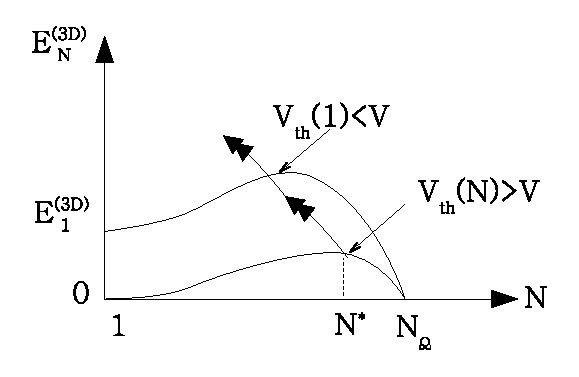
\includegraphics[width=0.8\columnwidth]{3dCondChange.eps}
	\caption{Condensation energy change with pair number  in 3D}
	\label{fig:3dCondChange}
\end{figure}

\section{Condensation energy for two pairs\label{sec:twoPair}}
The exact energy of two fermion pairs in the reduced BCS potential of Eq. (\ref{eq:VBcs}), has been shown to read as $E_2=R_1+R_2$ where $(R_1,R_2)$ are solution of the two Richardson-Gaudin equations
\begin{equation}
1=v\sum_{\vk}\frac{w_\vk}{2\epsilon_\vk-R_1}+\frac{2v}{R_1-R_2}=(R_{1}\leftrightarrow{}R_{2})
\label{eq:richardsonEq}
\end{equation}

If we now add and subtract these two equations, and use the single pair energy $\epsilon_{1}$ given in  Eq. (\ref{eq:onePair}), we rewrite this set equations without $v$, now hidden in $E_{1}$.  It reads 
\begin{gather}
\begin{split}
0=&(R_1-E_1)\sum_{\vk}\frac{w_\vk}{(2\epsilon_\vk-R_1)(2\epsilon_\vk-E_1)}\\
&+(R_{1}\leftrightarrow{}R_{2})\label{eq:2PairPlus}
\end{split}\\
-\frac{4}{(R_1-R_2)^2}=\sum_{\vk}\frac{w_\vk}{(2\epsilon_\vk-R_1)(2\epsilon_\vk-R_2)}\label{eq:2PairMinus}
\end{gather}

\subsection{Two pairs in 2D systems}
We have been able to solve these coupled equations analytically in the BCS case with a constant density of states above a frozen Fermi sea\cite{combescotBCS}.  We can use  this work  for 2D systems with a constant density of state with $w_\vk$ now equal to $1$ not for  for $0<\epsilon_k<\Omega$. The energy difference between two correlated pairs and two independent pairs reads in the large sample limit, as 
\begin{equation}
E^{\td}_2-2E_1^{\td}=\frac{2}{\rho}\left(1+\frac{2\sigma}{1-\sigma}\right)+\text{O}(\frac{1}{\rho^2})
\label{eq:}
\end{equation}
The $2/\rho$ contribution is the kinetic energy cost to add one pair when the density of state is constant while $[2/\rho][2\sigma/(1-\sigma)]$ is the change in the binding energy of two pairs induced by the moth-eaten effect. This result, far easier to obtain than the one for arbitrary $N$, not only gives the trend induced by Pauli blocking on the energy of $N$ correlated pairs, but also allows to obtain this energy exactly through a rule of the thumb that we have learned valid for all exciton problems we have studied up to now - excitons also are composite bosons with a many-body physics fully driven by Pauli blocking.  This rule says that, in the thermodynamical limit, i.e., large volume but $N/\rho$ constant, the result for $N$ is the result in 2 multiplied by $N-1$.  In the present case, this gives the energy change \emph{per pair}, $[E^{\td}_N-NE^{\td}_1]/N$, as $[(N-1)/\rho](1+\sigma)/(1-\sigma)$ in agreement with the result we have found through a far more complicated procedure than the ones to obtain the result for $N=2$.

\subsection{Two pairs in 3D system}
We now look for the solution of these two equations when the density of states is not constant but varies as $\rho\sqrt{\epsilon/\Omega}$.  Since the solution of these equations for $N=1$, i.e., without the term $2v/(R_1-R_2)$  in Eq. (\ref{eq:richardsonEq}), dramatically depends on the values of $\rho{}v$ compared to 1.

Let us first consider  $v\rho>1$.  A single pair then has a well defined bound state with $E_1$  finite. Since the change between the two pair energy $R_{1}+R_{2}$ and the energy of two single pairs  $2E_{1}$ can only come from Pauli blocking due to the very peculiar form of the reduced BCS potential, we expect $R_1+R_2\approx2E_1$, when $L^3\rightarrow\infty$, i.e., when $\rho\rightarrow\infty$. 

This can be understand more intuitively as such: a tight-binding state occupies large momentum-space with very small weight on each level. Therefore, Pauli blocking when introducing an extra pair is quite small as the occupation is much smaller than 1. Therefore, it is better energetically to put two pairs both in a state very like the original single-pair bound state than simply put the second pair in the next highest k-level as free Fermi gas.   

This leads to expand the sum n Eq. (\ref{eq:richardsonEq}) in terms of $(R_{1}-E_{1})$.  Using Eq. (\ref{eq:onepair}) for the first order term, we get
\begin{equation}
0=\sum_{n=1}^{\infty}(R_{1}-E_{1})^{n}\sum_{\vk}\frac{w_\vk}{(2\epsilon_\vk-E_1)^{(n+1)}}+\frac{2v}{R_1-R_2}
\end{equation}
If we now replace the sum over $\vk$ by an integral with a density of state $\rho\sqrt{\epsilon/\Omega}$, we can rewrite this sum as
\begin{multline}
\sum_{\vk}\frac{w_\vk}{(2\epsilon_\vk-E_1)^{(n+1)}}=\\\frac{\rho}{(-E_{1})^{n}}\sqrt{\frac{-E_{1}}{2\Omega}}K_{n}(\frac{2\Omega}{(-E_{1})})
\end{multline}
where $K_{n}$, defined as
\begin{equation}
K_{n}(x)\equiv\int_{0}^{x}\frac{\sqrt{y}\;dy}{2(y+1)^{n+1}}
\end{equation}
goes to $K_{n}$ when $x$ goes to infinity, which is the physical relevant limit since the simple pair binding energy is much smaller than the potential extension $\Omega$.

If we now rescale the $R_{i}$'s in terms of $E_{1}$ according to
\begin{equation}
R_{i}=E_{1}(1-t_{i})\quad\text{for }i=(1,2)
\end{equation}
the Richardson-Gaudin equations (\ref{eq:richardsonEq}) take a dimensionless form
\begin{equation}
0=\sum_{n=1}^{\infty}t_{1}^{n}K_{n}(\frac{2\Omega}{-E_{1}})+\frac{1}{\rho\Omega}\left(\frac{2\Omega}{-E_{1}}\right)^{3/2}\frac{1}{t_1-t_2}
\end{equation}

If we now add and subtract these two equations, we get
\begin{gather}
-\lambda^{2}=(t_{1}-t_{2})\sum_{n=1}^{\infty}(t_{1}^{n}-t_{2}^{n})K_{n}\label{eq:t1}\\
0=\sum_{n=1}^{\infty}(t_{1}^{n}+t_{2}^{n})K_{n}\label{eq:t2}
\end{gather}
when we have set $\lambda^{2/2}=(1/\rho\Omega)(2\Omega/(-E_{1}))^{3/2}$.

Two different regimes can then be distinguished.  
\begin{enumerate}
\item for $\lambda^{2}$ small compared to 1, Eq. (\ref{eq:t1}) gives $(t_{1}-t_{2})^{2}\approx-\lambda^{2}/K_{1}$. By writing $t_{1}^{2}+t_{2}^{2}$ as $\left[(t_{1}+t_{2})^{2}+t_{1}-t_{2})^{2}\right]$, Eq. (\ref{eq:t2}) then gives $t_{1}+t_{2})^{2}=\lambda^{2}K_{2}/2K_{1}^{2}$.  So that the dominant term of the two correlated pair energy in the large sample limit reads as 
\begin{equation}
E_{2}=R_{1}+R_{2}\approx2\left(E_{1}+\frac{1}{\rho}\sqrt{\frac{2\Omega}{-E_{1}}}\frac{K_{2}}{K_{1}^{2}}\right)
\end{equation}
$E_{2}$thus increases as $1/\rho\sim1/L^{3}$ with sample size.

To get the condensation energy, we have to compare this increase with the one of two free pairs.  Due to Pauli blocking, the momentum of the second pair is $2\pi/L$, so that the kinetic energy increase is $1/L^{2}$.  In the large $L$ limit, it is thus larger than the one of two correlated pair. 

As a result, the condensation energy per pair, which is the difference of the energy without and with potential, increases from 1 to 2 pairs - in agreement with our continuity argument. 

\item We now consider $\lambda^{2}$ larger than 1, which is reached for a single pair density energy $-E_{1}<\Omega^{1/3}/\rho^{2/3}\approx1/mL^{2}$.  In this regime, the single pair binding energy is smaller than the kinetic energy difference between the lowest free states. It is then no more possible to replace the sum over $\vk$ by a integral with a density of state.  So that the whole procedure to get the two pair energy fails.  

\end{enumerate}

Let us now tackle the two-pair energy at threshold for one pair and ??? that indeed, the sum over $\vk$ cannot be replaced by an integral for the lowest $\vk$'s.
Let us start with the threshold case $v=v_{\text{th}}(1)$, i.e., $v\rho=1$.  We then have $S(E=0)=1$, so that the Richardson-Gaudin equations also read, for $R_1=R+iR'$
\begin{equation}
\sum\frac{w_\vk}{2\epsilon_\vk}=\sum\frac{w_\vk}{2\epsilon_\vk-R-iR'}-\frac{i}{R'}
\label{eq:}
\end{equation}
This equation splits into two equations, for the real and imaginary parts

The problem then is to find $R$ solution of 
\begin{equation}
\sum\frac{w_\vk}{2\epsilon_\vk}=\sum{}w_\vk\frac{2\epsilon_\vk-R}{(2\epsilon_\vk-R)^2+R'^2}
\label{eq:}
\end{equation}
where $R'$ such that 
\begin{equation}
R'^2\sum{}\frac{w_\vk}{(2\epsilon_\vk-R)^2+R'^2}=1
\label{eq:R'}
\end{equation}
in the large sample limit, i.e., the dominate term of the $\rho$ dependence of $R$ when $1/\rho$ goes to zero. 

By combining these two equation, we get
\begin{equation}
R\sum{}w_\vk\frac{2\epsilon_\vk-R}{(2\epsilon_\vk-R)^2+R'^2}=1
\label{eq:R}
\end{equation}

A possible trick to solve these equations is to note that $\sum_\vk{}w_\vk=N_\Omega=\frac23\rho\Omega$ in 3D (which it is $\rho\Omega$ in 2D).  This allows to rewrite Eqs. (\ref{eq:R'},\ref{eq:R})
\begin{gather}
\sum{}w_\vk\left[\frac{1}{(2\epsilon_\vk-R)^2+R'^2}-\frac{1}{N_\Omega{}R'^2}\right]=0\\
\sum{}w_\vk\left[\frac{2\epsilon_\vk-R}{(2\epsilon_\vk-R)^2+R'^2}-\frac{1}{N_\Omega{}R}\right]=0
\end{gather}
This readily shows that if $R$ and $R'$ were finite when $\rho\rightarrow\infty$, i.e., these questions cannot be fulfilled because we 
................................



\section{Conclusion\label{sec:conclusion}}
The upper energy cutoff $\Omega$ for the phase space in our model seems quite arbitrary.  After all, real system has no such cutoff and they have infinite amount of high-momentum states to use.   It seems a little dubious that condensation energy vanishes when all states below $\Omega$ is filled.  On the other hand, this fact can be interpret in such way:  energy cutoff $\Omega$ is introduced because we take potential as constant and ignore the fall-off of the potential in high energy.  The amplitude of potential defines an energy scale, which in turn defines a region in phase space.  Beyond this space, potential is too small and does not affect the distribution of fermions and fermions pack themselves just as free gas, therefore equivalently gives zero condensation-energy. 

We present an analysis about the transition from one-pair and many-pair with the same hamiltonian within Richardson-Gaudin equations framework.  We observe that condensation energy increases in the beginning and decreases toward the full filling. When attraction is small enough, there is no bound state for single pair, but later, fermions formed a many-body bound state and lower the system energy, when fermion number further increases, system gets back into the normal state as free Fermi gas.  By utilizing Richardson-Gaudin equations in canonical ensemble, we illustrate the intricacy of the many-body state of superconductivity.  

One of us (M.C.) wishes to thank the University of Illinois at
Urbana-Champaign, and Tony Leggett in particular, for enlightening discussions during her invitations at
the Institute for Condensed Matter Physics where most of the present work has been
performed. 
 
 
\appendix
\section{Scattering amplitude and scattering length for our model \label{sec:scatter}}
In dilute system or short-range potential, low-energy property of the potential can be described with scattering amplitude\cite{Pethick,Fetter}, more specifically, s-wave scattering length $a_{s}$ is routinely used to describe the potential in atomic physics, where most problems is only about very low energy and low density.  So it is interesting to find the scattering amplitude and s-wave scattering length for our model potential (Eq. (\ref{eq:VBcs})). We notice that our model is actually very similar as the one-channel model used by Gurarie and Radzihovsky (sec. 3 and sec. 4.1 of Ref. \cite{GurarieNarrow}). 

Scattering amplitude, or, T-matrix can be written as 
\begin{equation}
\frac{4\pi}{m}f_{\vk\vk'}=T_{\vk\vk'}=[\frac{U}{(1-U\Pi)}]_{\vk\vk'}
\end{equation}
where $\Pi$ is the propagator of a pair.  In a translation invariant system with central potential, all quantities depend $\vk$ and $\vk'$ only through $\vk-\vk'$ and we can separate the solution into different partial wave. Especially for the s-wave, the complicated  integral becomes a simple number,
\begin{equation}
T^{0}_{k}=\frac{u^{0}_{k}}{1-u^{(0)}_{k}\Pi^{(0)}(\epsilon_k)}
\end{equation}
Here 
\begin{equation}
\begin{split}
\Pi^{(0)}(\epsilon)=&\int\frac{d^{3}\vq}{{(2\pi)}^{3}}\frac{w_{k}}{\epsilon-q^{2}/m+i0}\\
=&-\frac{m}{2\pi^{2}}{\Lambda}+\frac{m\sqrt{\epsilon{m}}}{2\pi^{2}}\arctan\frac{\Lambda}{\sqrt{\epsilon{m}}}\\
&-i\frac{m^{3/2}}{4\pi}\sqrt{\epsilon}
\end{split}
\end{equation}
Where $\Lambda$ is the cutoff in momentum, $\Lambda^{2}/(2m)\equiv\Omega$. The second term is small compared to the first term when the cutoff is large, so we will ignore it.  In our model, $u^{0}_{k}=-vw_{k}$, And we find the scattering amplitude 
\begin{equation}
f_{s}(k)=-\frac{1}{-\frac{4\pi}{mv}+\frac{2\Lambda}{\pi}+ik}
\end{equation}
and s-wave scattering length is its limit at zero energy. 
\begin{equation}
\begin{split}
a(v)=&\left(-\frac{4\pi}{mv}+\frac{2\Lambda}{\pi}\right)^{-1}\equiv\frac{m}{4\pi}v_{R}\\
     =&\frac{m}{4\pi}\frac{-v}{1-v/v_{c}}
     \end{split}
\end{equation}
where $v_{R}$ can be called renormalized coupling and 
\begin{equation}
v_{c}=\frac{2\pi^{2}}{\Lambda{m}}
\end{equation}
We find that, for large attractive, i.e., for $v$ large and position, $a\approx\frac{m}{4\pi}v_c$ is small positive as $\Lambda$ is large and increases as attraction decrease, it diverges at $v=v_{c}$ and which is the same as our threshold $v^{\text{th}}(1)$.  When $v$ gets even smaller, there is no bound-state and $a$ becomes large negative and its absolute value decease as $v$ decrease until $a(v=0)=0$. 
$a(v)$ can also be written as
\begin{equation}
a(v)=\frac{\pi}{2\Lambda}\left(1-\frac{2\pi^{2}}{mv\Lambda}\right)^{-1}
\end{equation}
This can be easily related to binding energy Eq. (\ref{eq:E3Dsmall}) by $E_{b}=-1/(ma^{2})$ when close to threshold. 


\begin{thebibliography}{18}
\expandafter\ifx\csname natexlab\endcsname\relax\def\natexlab#1{#1}\fi
\providecommand{\bibinfo}[2]{#2}
\ifx\xfnm\relax \def\xfnm[#1]{\unskip,\space#1}\fi
%Type = Article
\bibitem[{Cooper(1956)}]{Cooper}
\bibinfo{author}{L.~N. Cooper}, \bibinfo{journal}{Phys. Rev.}
  \bibinfo{volume}{104} (\bibinfo{year}{1956}) \bibinfo{pages}{1189--1190}.
%Type = Article
\bibitem[{Bardeen et~al.(1957)Bardeen, Cooper, and Schrieffer}]{BCS}
\bibinfo{author}{J.~Bardeen}, \bibinfo{author}{L.~N. Cooper},
  \bibinfo{author}{J.~R. Schrieffer}, \bibinfo{journal}{Phys. Rev.}
  \bibinfo{volume}{106} (\bibinfo{year}{1957}) \bibinfo{pages}{162}.
%Type = Article
\bibitem[{{Gor'kov} and Melik-Barkhudarov(1962)}]{Gorkov}
\bibinfo{author}{L.~P. {Gor'kov}}, \bibinfo{author}{T.~K. Melik-Barkhudarov},
  \bibinfo{journal}{Sov. Phys. JETP} \bibinfo{volume}{13}
  (\bibinfo{year}{1962}) \bibinfo{pages}{1018--1022}.
%Type = Article
\bibitem[{Eagles(1969)}]{Eagle}
\bibinfo{author}{D.~M. Eagles}, \bibinfo{journal}{Phys. Rev.}
  \bibinfo{volume}{186} (\bibinfo{year}{1969}) \bibinfo{pages}{456--463}.
%Type = Inproceedings
\bibitem[{Leggett(1980)}]{LeggettCrossover}
\bibinfo{author}{A.~J. Leggett}, in: \bibinfo{booktitle}{Proceedings of the
  XVIth Karpacz Winter School of Theoretical Physics, Karpacz, Poland},
  \bibinfo{publisher}{Springer-Verlag}, \bibinfo{year}{1980}, pp.
  \bibinfo{pages}{13--27}.
%Type = Article
\bibitem[{Nozi\`{e}res and Schmitt-Rink(1985)}]{Nozieres}
\bibinfo{author}{P.~Nozi\`{e}res}, \bibinfo{author}{S.~Schmitt-Rink},
  \bibinfo{journal}{Journal of Low Temperature Physics} \bibinfo{volume}{59}
  (\bibinfo{year}{1985}) \bibinfo{pages}{195--211}.
  \bibinfo{note}{10.1007/BF00683774}.
%Type = Article
\bibitem[{Richardson(1963)}]{Richardson1}
\bibinfo{author}{R.~W. Richardson}, \bibinfo{journal}{physics letters}
  \bibinfo{volume}{3} (\bibinfo{year}{1963}) \bibinfo{pages}{277--279}.
%Type = Article
\bibitem[{Richardson and Sherman(1964)}]{Richardson2}
\bibinfo{author}{R.~W. Richardson}, \bibinfo{author}{N.~Sherman},
  \bibinfo{journal}{Nucl. Phys.} \bibinfo{volume}{52} (\bibinfo{year}{1964})
  \bibinfo{pages}{221--238}.
%Type = Article
\bibitem[{Richardson(1977)}]{Richardson3}
\bibinfo{author}{R.~W. Richardson}, \bibinfo{journal}{Journal of Mathematical
  Physics} \bibinfo{volume}{18} (\bibinfo{year}{1977}) \bibinfo{pages}{1802}.
%Type = Article
\bibitem[{Richardson(1968)}]{Richardson1968}
\bibinfo{author}{R.~W. Richardson}, \bibinfo{journal}{Journal of Mathematical
  Physics} \bibinfo{volume}{9} (\bibinfo{year}{1968}) \bibinfo{pages}{1327}.
%Type = Book
\bibitem[{Gaudin(1995)}]{gaudin}
\bibinfo{author}{M.~Gaudin}, \bibinfo{title}{{\'{E}tats Propres et Valeurs
  Propres de l'Hamiltonien d'Appariement}}, \bibinfo{publisher}{Les
  \'{E}ditions de Physique, France}, \bibinfo{year}{1995}.
%Type = Article
\bibitem[{Combescot et~al.(2008)Combescot, Betbeder-Matibet, and
  Dubin}]{CobosonPhysicsReports}
\bibinfo{author}{M.~Combescot}, \bibinfo{author}{O.~Betbeder-Matibet},
  \bibinfo{author}{F.~Dubin}, \bibinfo{journal}{Physics Reports}
  \bibinfo{volume}{463} (\bibinfo{year}{2008}) \bibinfo{pages}{215}.
%Type = Article
\bibitem[{{Combescot} and {Zhu}(2010)}]{CobosonBcsRich}
\bibinfo{author}{M.~{Combescot}}, \bibinfo{author}{G.~{Zhu}},
  \bibinfo{journal}{Eur.Phys.J.B,}  (\bibinfo{year}{2010}). \bibinfo{note}{To
  be published}.
%Type = Unpublished
\bibitem[{Pogosov and Combescot(2009)}]{CombescotCooper}
\bibinfo{author}{W.~V. Pogosov}, \bibinfo{author}{M.~Combescot},
  \bibinfo{title}{A striking understanding of cooper pair energy},
  \bibinfo{year}{2009}. \bibinfo{note}{To be published}.
%Type = Article
\bibitem[{Pogosov et~al.(2010)Pogosov, Combescot, and Crouzeix}]{combescotBCS}
\bibinfo{author}{W.~V. Pogosov}, \bibinfo{author}{M.~Combescot},
  \bibinfo{author}{M.~Crouzeix}, \bibinfo{journal}{Phys. Rev. B}
  \bibinfo{volume}{81} (\bibinfo{year}{2010}) \bibinfo{pages}{174514}.
%Type = Book
\bibitem[{Pethick and Smith(2001)}]{Pethick}
\bibinfo{author}{C.~J. Pethick}, \bibinfo{author}{H.~Smith},
  \bibinfo{title}{{Bose-{E}instein Condensation in Dilute Gases}},
  \bibinfo{publisher}{Cambridge University Press}, \bibinfo{year}{2001}.
%Type = Book
\bibitem[{Fetter and Walecka(1971)}]{Fetter}
\bibinfo{author}{A.~L. Fetter}, \bibinfo{author}{J.~D. Walecka},
  \bibinfo{title}{{Quantum Theory of Many-Particle Systems}},
  \bibinfo{publisher}{Dover Publications, Inc. (Original Publisher:
  McGraw-Hill)}, \bibinfo{edition}{dover} edition, \bibinfo{year}{1971}.
%Type = Article
\bibitem[{Gurarie and Radzihovsky(2007)}]{GurarieNarrow}
\bibinfo{author}{V.~Gurarie}, \bibinfo{author}{L.~Radzihovsky},
  \bibinfo{journal}{Annals of Physics} \bibinfo{volume}{322}
  (\bibinfo{year}{2007}) \bibinfo{pages}{2 -- 119}. \bibinfo{note}{January
  Special Issue 2007}.

\end{thebibliography}

\end{document}
